% This file was created by matplotlib2tikz v0.6.17.
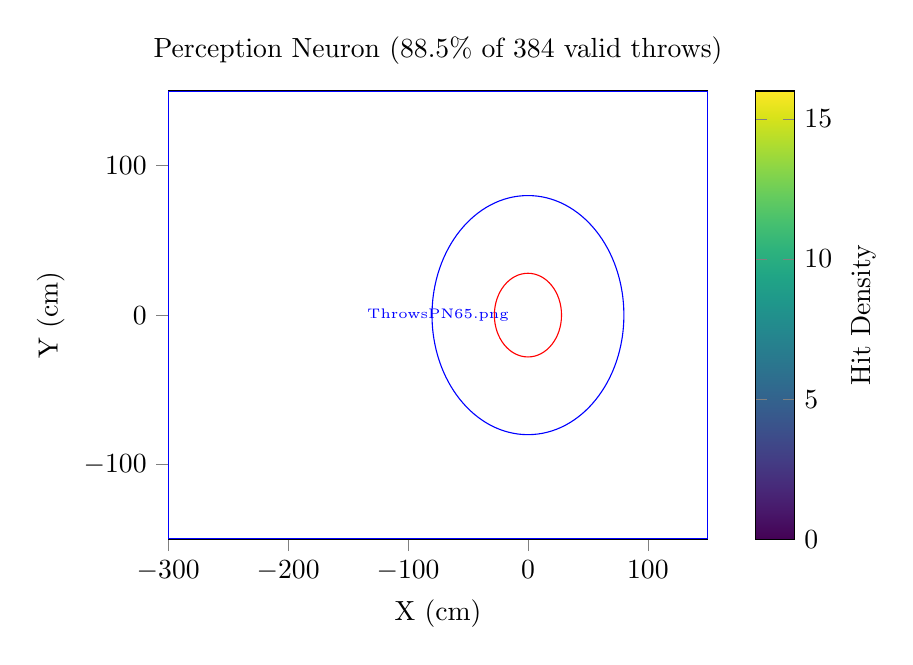
\begin{tikzpicture}

\begin{axis}[
title={Perception Neuron (88.5\% of 384 valid throws)},
xlabel={X (cm)},
ylabel={Y (cm)},
xmin=-300, xmax=150,
ymin=-150, ymax=150,
tick align=outside,
tick pos=left,
x grid style={white!69.019607843137251!black},
y grid style={white!69.019607843137251!black},
colorbar,
colormap/viridis,
point meta min=0,
point meta max=16,
colorbar style={ylabel={Hit Density}}
]
\addplot graphics [includegraphics cmd=\pgfimage,xmin=-300, xmax=150, ymin=-150, ymax=150] {ThrowsPN65.png};
\draw[draw=white,fill opacity=0] (axis cs:0,0) circle (130);
\draw[draw=blue,fill opacity=0] (axis cs:0,0) circle (80);
\draw[draw=red,fill opacity=0] (axis cs:0,0) circle (28);
\draw[draw=white,fill opacity=0] (axis cs:0,0) circle (5);
\draw[draw=white,fill=white] (axis cs:-220,-50) circle (5);
\end{axis}

\end{tikzpicture}